\documentclass[11pt,aspectratio=169,handout]{beamer}

\usetheme{Singapore}
\usecolortheme{orchid}

\usepackage[utf8]{inputenc}
\usepackage[russian]{babel}
\usepackage{amsmath}
\usepackage{amsfonts}
\usepackage{amssymb}
\usepackage{graphicx}
\usepackage{bibentry}
\usepackage{wasysym}
\usepackage[most]{tcolorbox}
\usepackage[normalem]{ulem}

\usepackage{hyperref}

\definecolor{info}{RGB}{62, 180, 137}
\definecolor{warn}{RGB}{128, 0, 0}

\author{Николай Анохин}
\title{Рекомендательные сервисы в продакшене}

\titlegraphic{
   
\includegraphics[width=.07\textwidth]{images/ok_logo.png}
   
\includegraphics[width=.07\textwidth]{images/made_logo.png}
}

\AtBeginSection[]{
  \begin{frame}
  \vfill
  \centering
  \begin{beamercolorbox}[sep=8pt,center,shadow=true,rounded=true]{title}
    \usebeamerfont{title}\insertsectionhead\par
  \end{beamercolorbox}
  \vfill
  \end{frame}
}

%\setbeamercovered{transparent} 
%\setbeamertemplate{navigation symbols}{} 
%\logo{} 
%\institute{} 
%\date{} 
%\subject{} 

\begin{document}

{
\setbeamertemplate{headline}{}

\begin{frame}
\titlepage
\end{frame}

%\begin{frame}
%\tableofcontents
%\end{frame}

}

\begin{frame}{}

\begin{tcolorbox}[colback=info!5,colframe=info!80,title=Входной опрос]
\url{https://forms.gle/vBpRB7UAHxtzCA1X8}
\end{tcolorbox}

\end{frame}

\section{Информация о курсе}

\begin{frame}{Николай Анохин}

\begin{center}
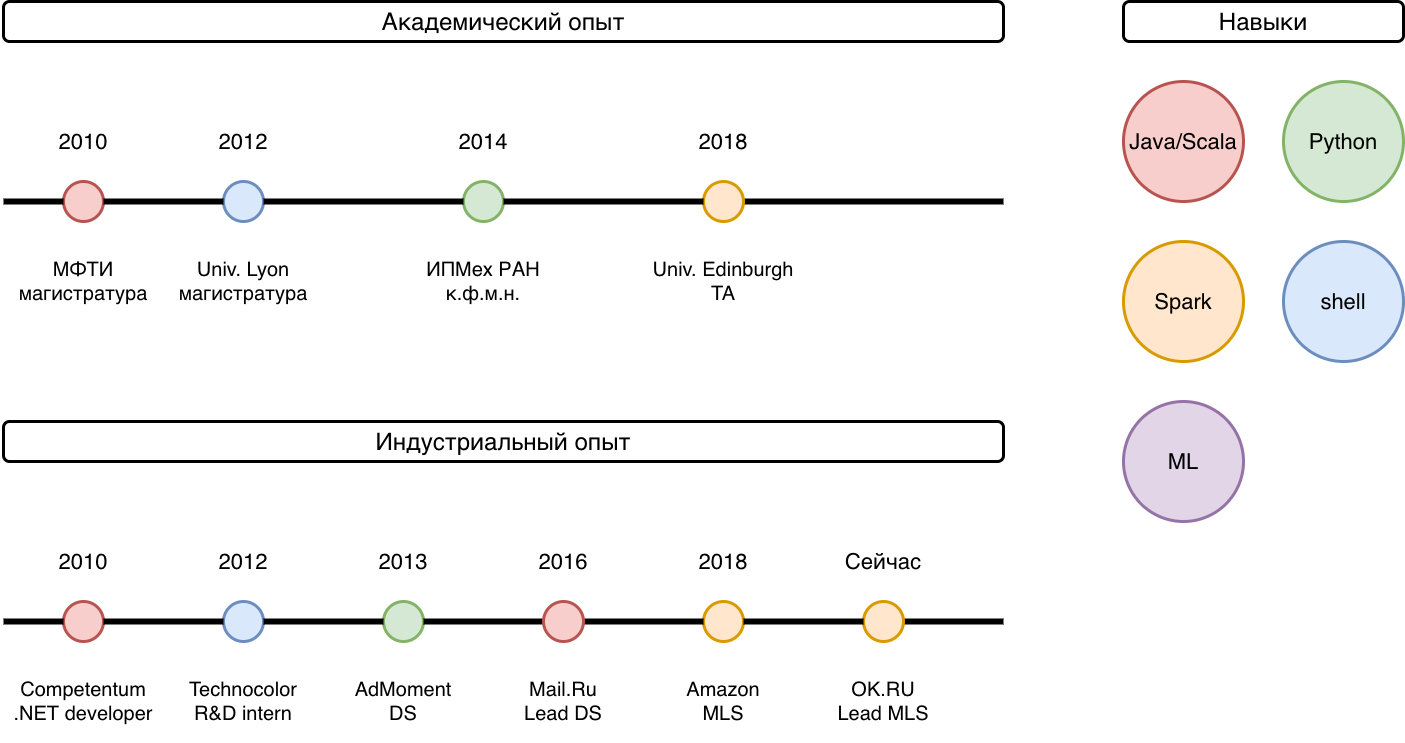
\includegraphics[scale=0.23]{images/about-me.png}
\end{center}

\end{frame}

\begin{frame}{Дарья Никанорова}

\begin{center}
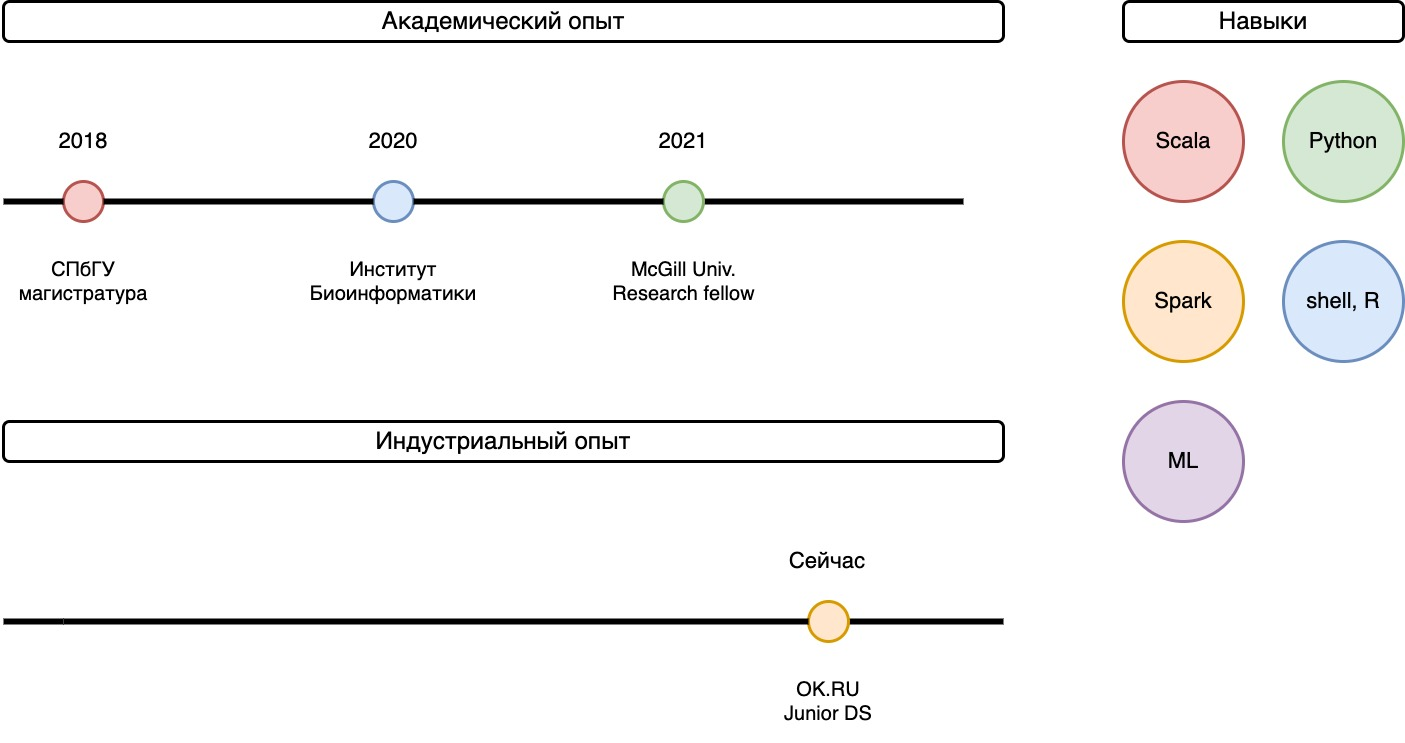
\includegraphics[scale=0.23]{images/about-me-dasha.jpg}
\end{center}

\end{frame}

\begin{frame}{Discord}

Канал курса: \url{https://TODO}

\vfill

\begin{itemize}
\item Вопросы вне занятия можно задать в личке или в чате курса (лучше)
\item Тегайте нас, чтобы мы не пропустили ваш комментарий в общем потоке сообщений
\item Если ответа не последовало в течении 24 часов, то мы, вероятно, не увидели ваше сообщение. Не стесняйтесь его продублировать
\end{itemize}

\end{frame}

\begin{frame}{Как задать вопрос}

\begin{itemize}
\item Голосом
\item В специально выделенное для этого время
\item Перед тем как спросить будет хорошим тоном поставить несколько знаков вопроса
\begin{tcolorbox}[colback=gray!5,colframe=gray!80,title=]
20:23 Саша: ???? \\
20:23 Преподаватель: Ждём вопроса от Саши \\
20:24 Саша: Какая метрика хорошо работает в задаче рекомендаций?
\end{tcolorbox}
\end{itemize}

\end{frame}

\begin{frame}{Если что-то пошло не так}

\begin{itemize}
\item Пропал голос
\item Исчезло изображение
\item Плохо слышно
\item Любые проблемы другого характера
\end{itemize}
\vfill
{\bf Сразу пишем в чат} много минусов и не ждем других участников. Если вы увидели, что в чате кто-то написал много минусов, а у вас всё хорошо, то поставьте несколько плюсов:
\vfill
\begin{tcolorbox}[colback=gray!5,colframe=gray!80,title=]
20:24 Петя: - - - - - - -  \\
20:25 Саша: ++++ \\
20:25 Ольга: +++++++
\end{tcolorbox}

\end{frame}

\begin{frame}{Программа модуля}
\begin{small}
\begin{tabular}{ l | l | c | c | c }
{\bf Дата} & {\bf Тема} & {\bf Квиз} & {\bf Семинар} & {\bf Домашка} \\
\hline
2022-05-19 & Рекомендательные сервисы в продакшене & \checked  & \checked &  \\
2022-05-26 & Метрики и базовые подходы & \checked  &  \checked &  \\ 
2022-06-02 & Классические алгоритмы & \checked  & \checked & \checked  \\
2022-06-09 & Нейросетевые рекомендеры & \checked  & \checked &  \\
2022-09-16 & Нерешенные проблемы и новые направления & \checked  &  \checked &
\end{tabular}
\end{small}

\vfill

Репозиторий на GH: \url{https://github.com/anokhin/recsys-made-2022}

\end{frame}

\begin{frame}{Оценка $\in [0, 1]$}

\begin{itemize}
\item Идеальное выполнение квизов и домашки = нижняя граница ``пятерки''
\item Дополнительные баллы можно получить на зачете
\item Выберем трех самых активных слушателей и накинем им по 0.1
\end{itemize}

\end{frame}

\begin{frame}{Пройдя этот курс, вы...}

\begin{itemize}
\item Разработаете свой рекомендательный сервис (почти) с нуля
\item Сможете выбирать правильные инструменты под конкретную задачу
\item Узнаете о проблемах, возникающих в боевых RS, и научитесь их решать
\item Будете в курсе SOTA моделей и задач RS, над которыми работают ученые
\end{itemize}

\end{frame}

\section{Зачем нужны рекомендательные сервисы}

\begin{frame}{}

\vfill
\begin{tcolorbox}[colback=info!5,colframe=info!80,title=]
{\bf Recommender Systems} (RS) are software tools and techniques providing suggestions for {\bf items} to be of use to a {\bf user} \cite{RSHB}.
\end{tcolorbox}
\vfill
\begin{center}
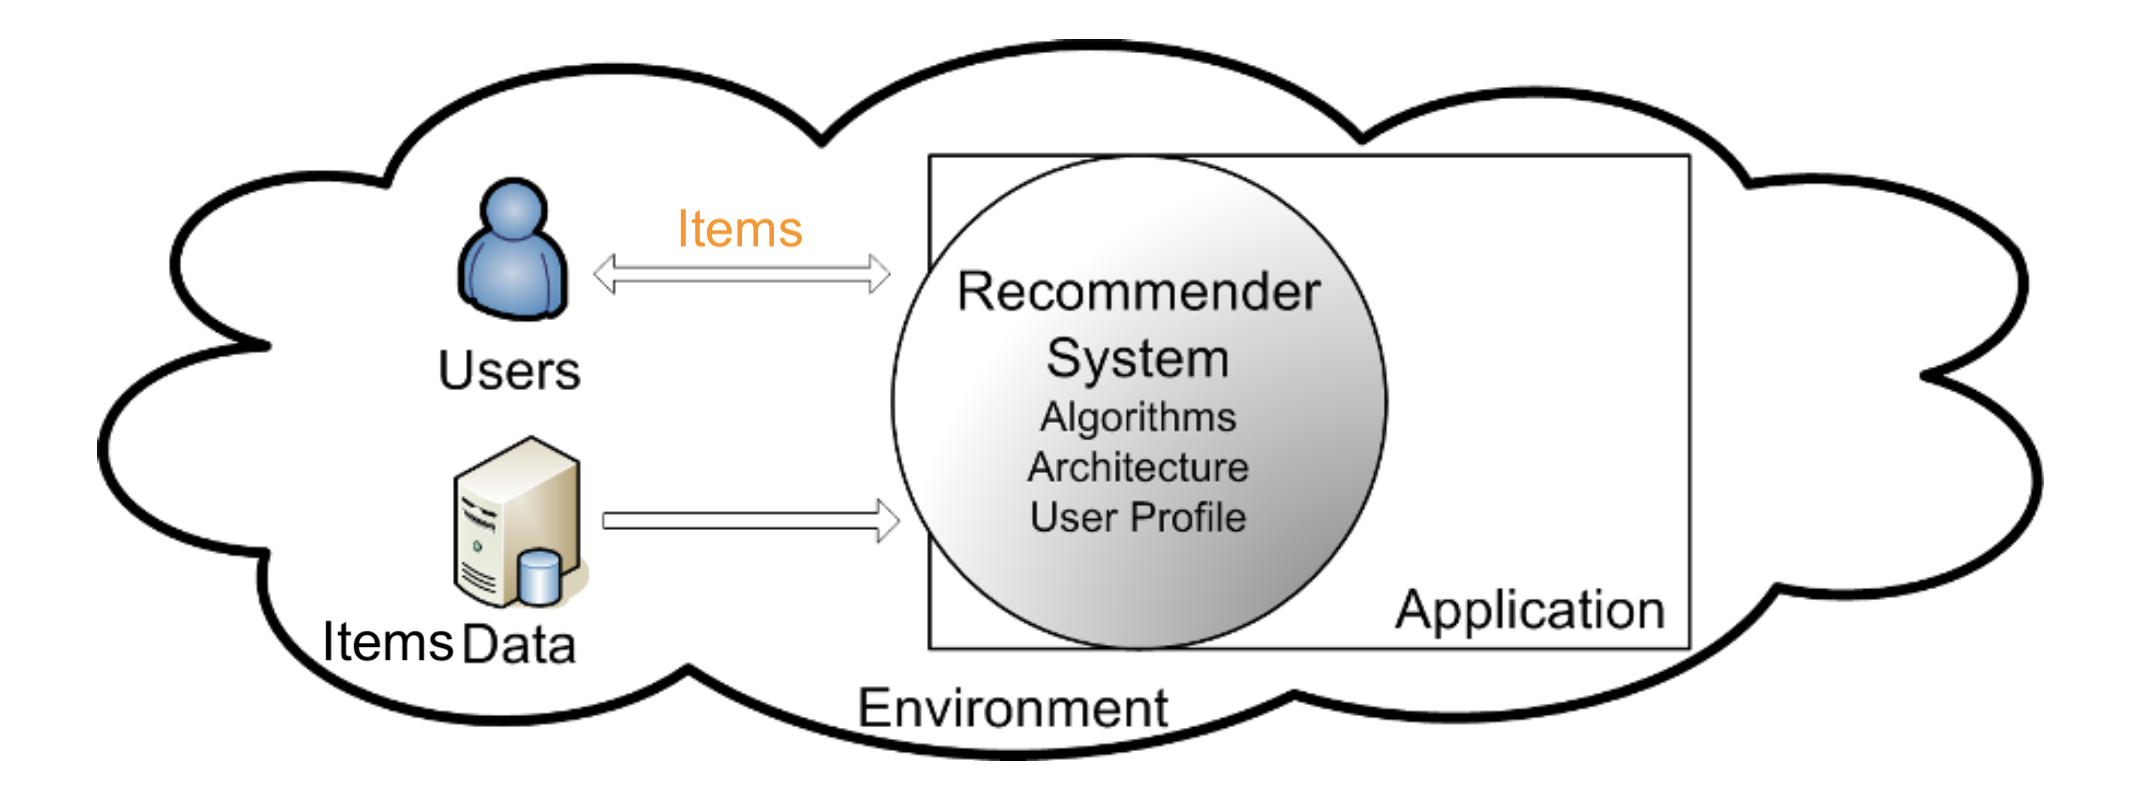
\includegraphics[scale=0.3]{images/overall.png}
\end{center}

\end{frame}

\begin{frame}{}

\begin{center}
\includegraphics[scale=0.25]{images/netflix-0.png}
\end{center}

\end{frame}

\begin{frame}{}

\begin{center}
\includegraphics[scale=0.25]{images/netflix-1.png}
\end{center}

\end{frame}

\begin{frame}{}

\begin{center}
\includegraphics[scale=0.25]{images/netflix-2.png}
\end{center}

\end{frame}

\begin{frame}{}

\begin{center}
\includegraphics[scale=0.25]{images/netflix-3.png}
\end{center}

\end{frame}

\begin{frame}{}

\begin{center}
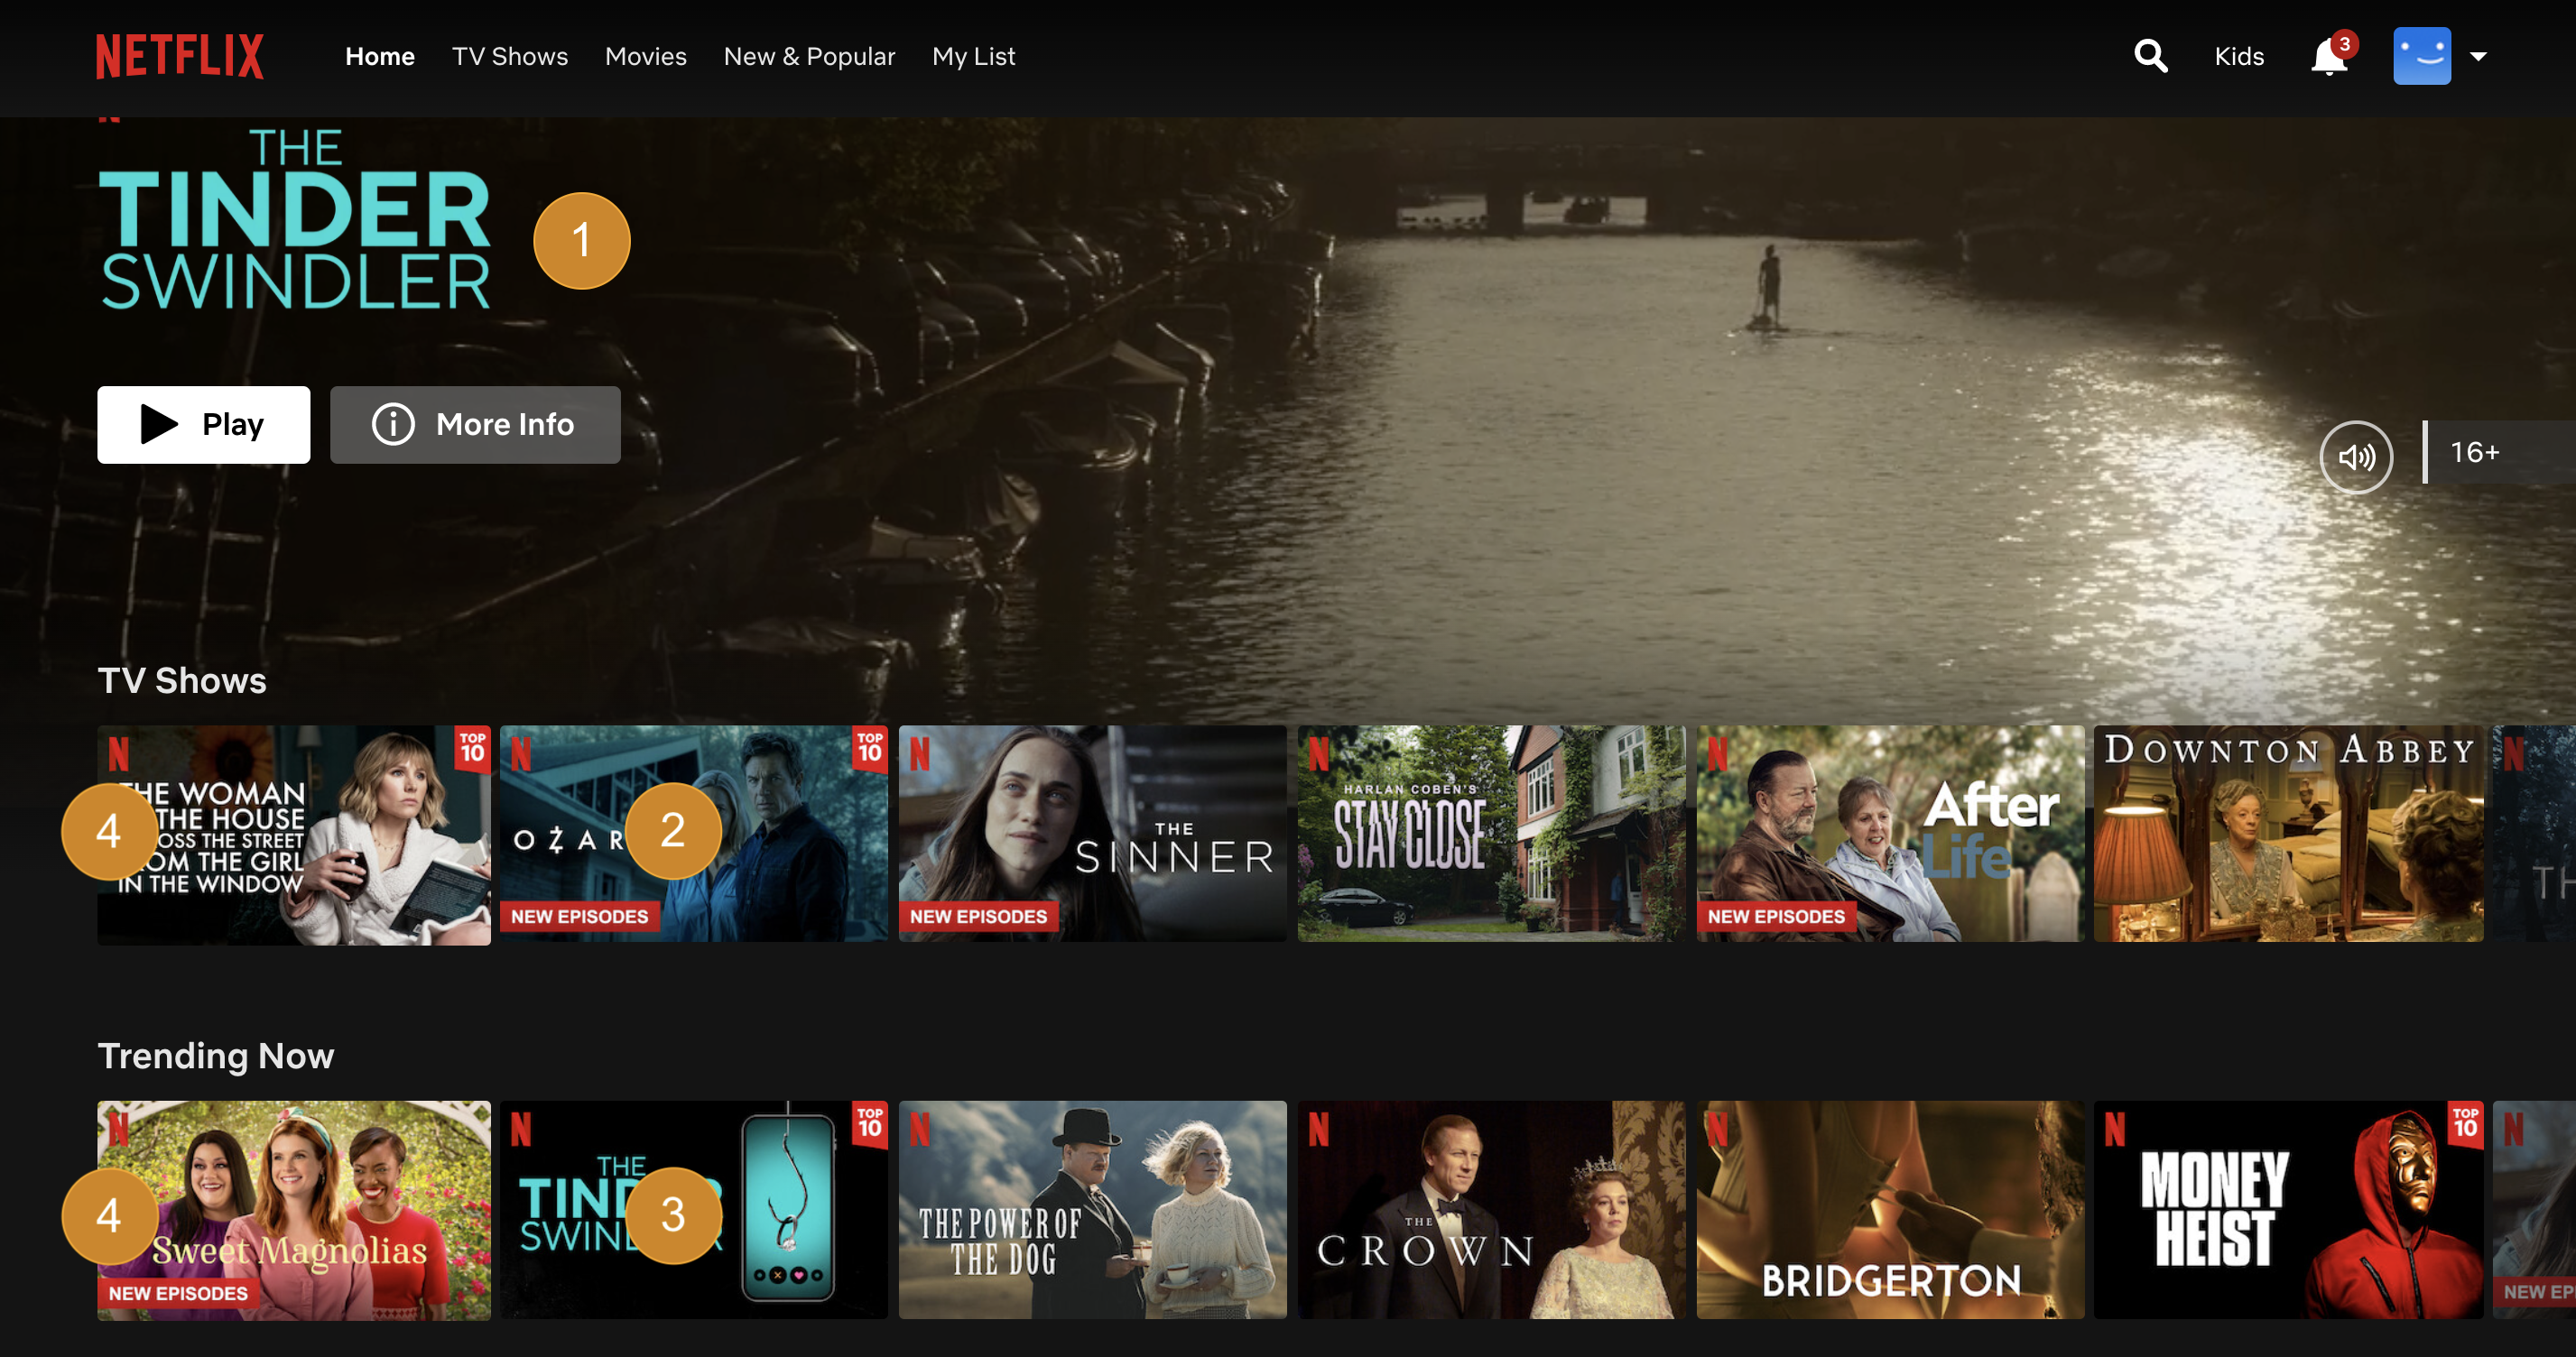
\includegraphics[scale=0.25]{images/netflix-4.png}
\end{center}

\end{frame}

\begin{frame}{}

\begin{center}
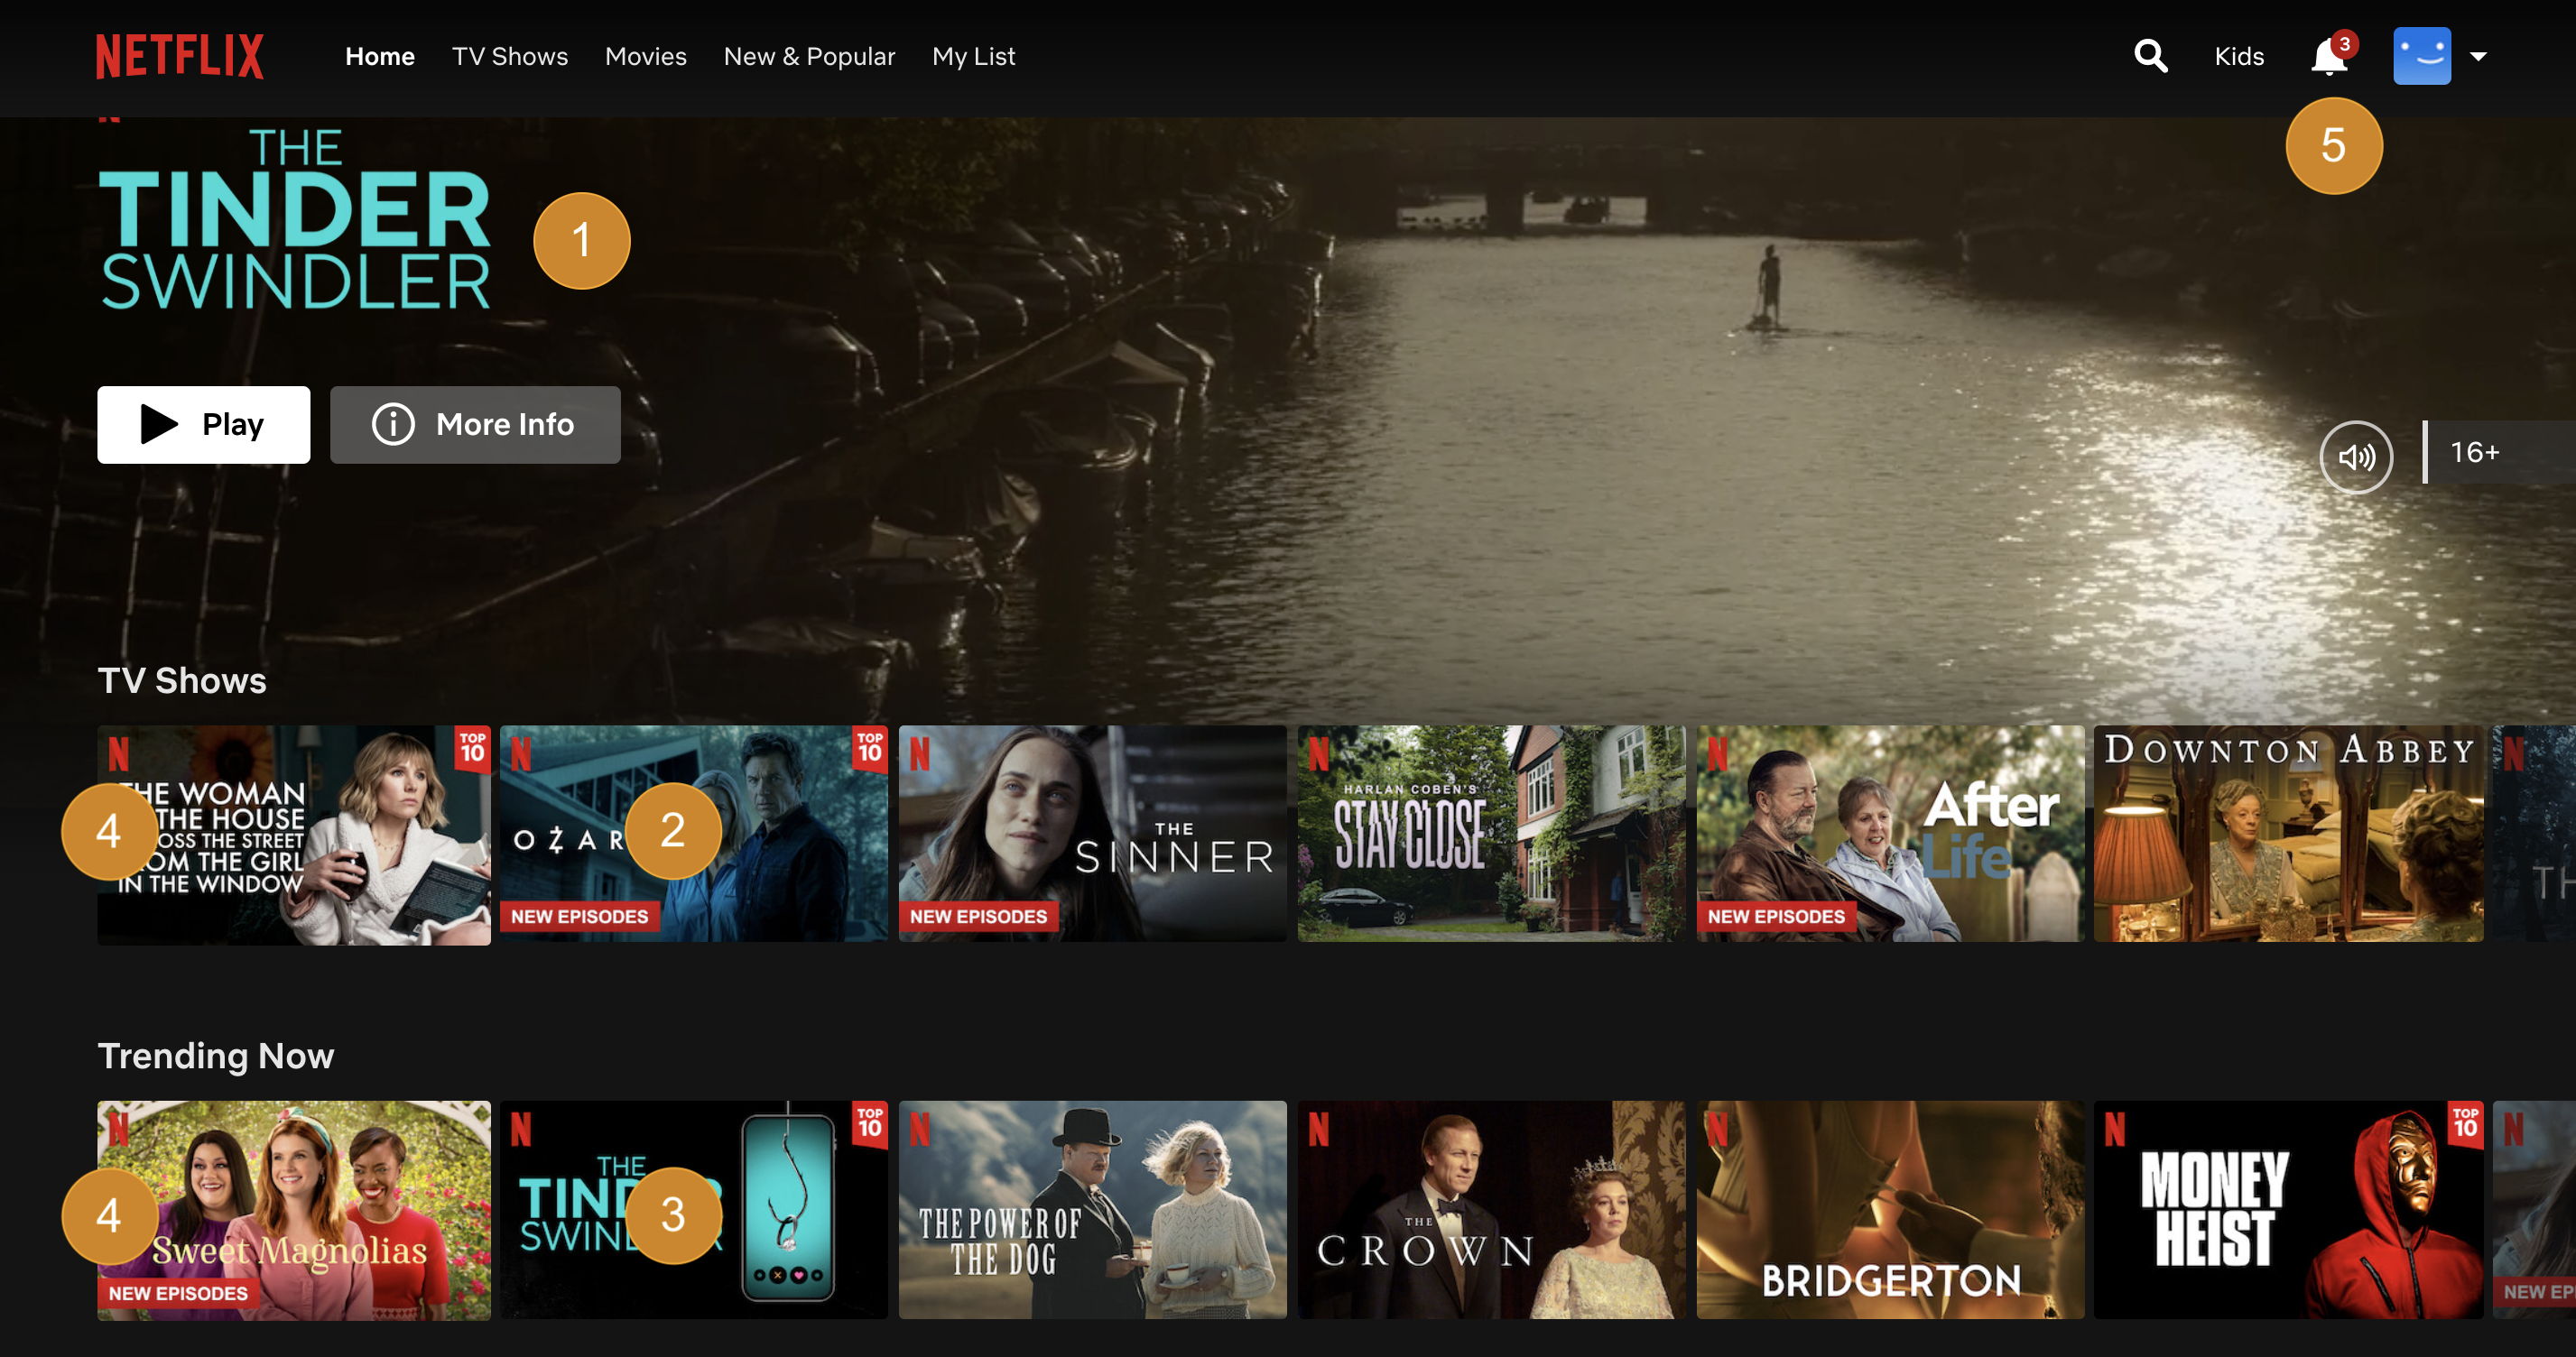
\includegraphics[scale=0.25]{images/netflix-5.png}
\end{center}

\end{frame}

\begin{frame}{}

\begin{center}
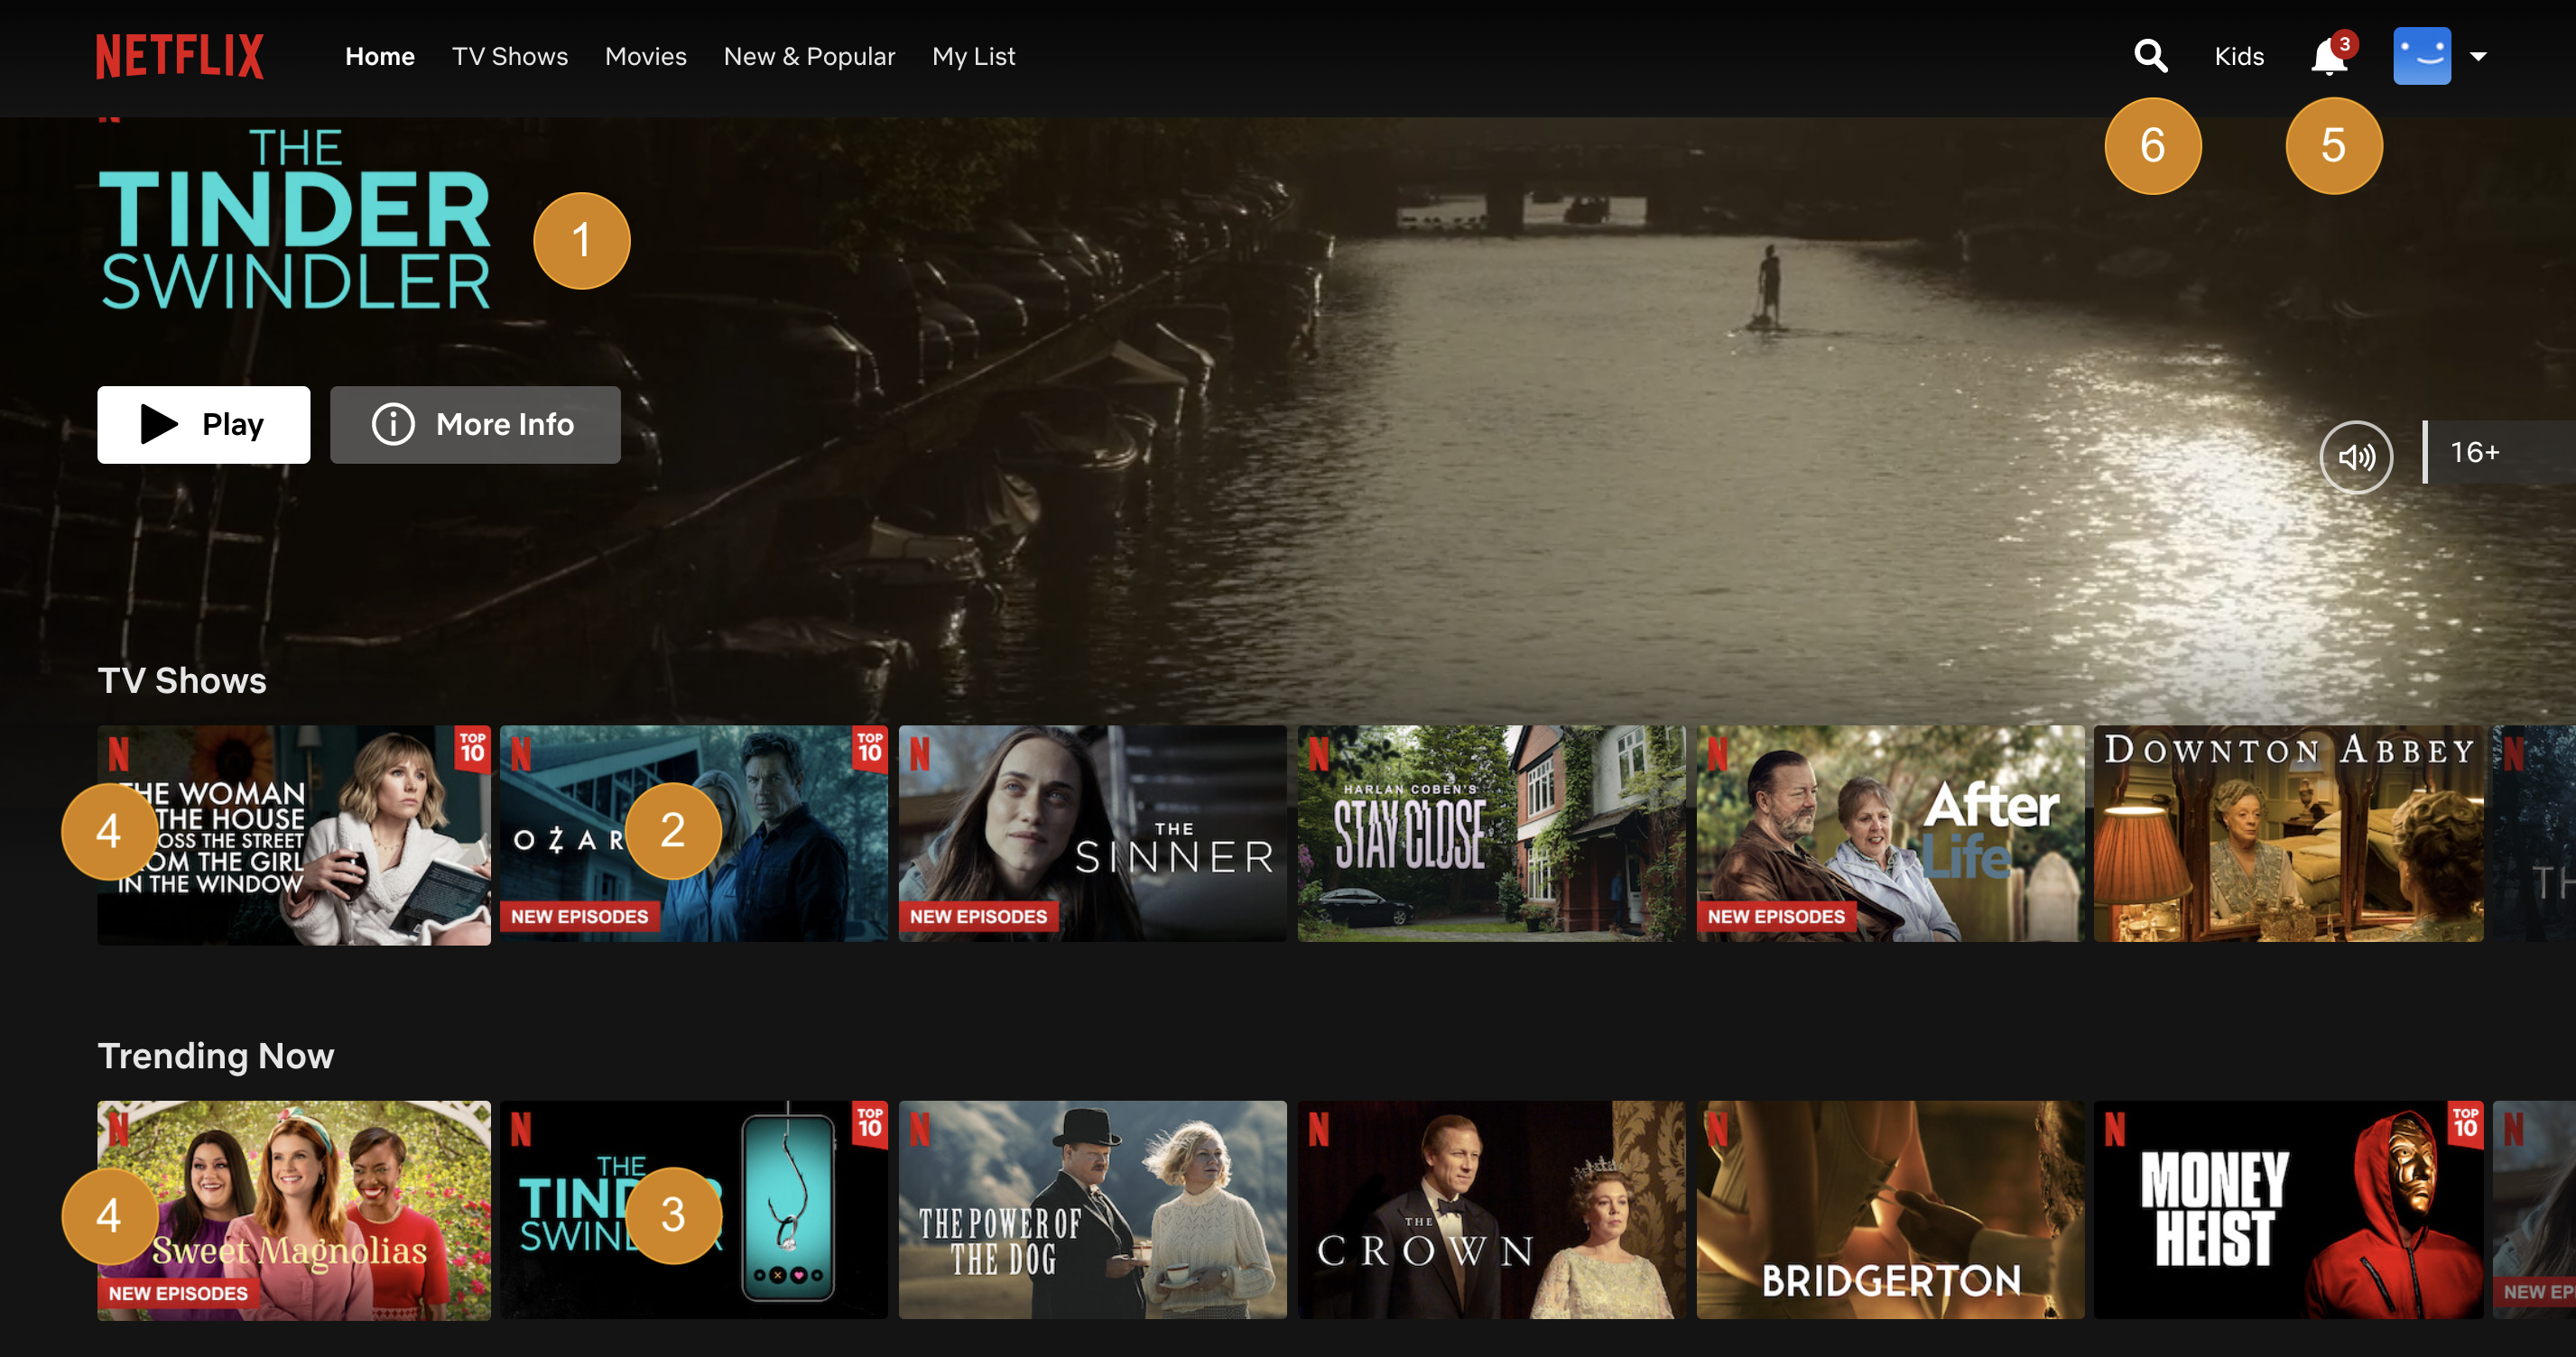
\includegraphics[scale=0.25]{images/netflix-6.png}
\end{center}

\end{frame}

\begin{frame}{RS vs другие задачи ML \cite{NETFLIX}}

\begin{itemize}[<+->]
\item RS ориентированы на продакшен
\item Наблюдаемые данные очень разреженные
\item Наблюдаем разное количество данных в зависимости от популярности
\item Отсутствующие данные -- либо ненаблюдаемые позитивные, либо негативные
\item Отсутствующие данные -- missing not-at-random
\item Рекомендательные сервисы живут в петле обратной связи
\end{itemize}

\end{frame}

\begin{frame}{Зачем RS бизнесу}

\begin{itemize}[<+->]
\item Увеличить продажи
\item Продвигать более разнообразные айтемы
\item Улучшить пользовательский опыт
\item Добиться большей лояльности
\item Лучше понимать пользователей
\end{itemize}

\end{frame}

\begin{frame}{Зачем RS пользователям}

\begin{itemize}[<+->]
\item Найти лучший товар
\item Найти {\bf все} подходящие товары
\item Найти последовательность или набор товаров
\item Залипнуть
\item Найти рекомендер, которому можно доверять
\item Реализовать творческие потребности
\item Помочь другим сделать выбор
\end{itemize}

\end{frame}

\begin{frame}{Зачем RS инженерам}

\begin{itemize}
\item Делать высоконагруженный отказоустойчивый сервис
\item Анализировать большие данные
\item Окунуться в волшебный мир \sout{матана} машинного обучения
\item Объективно измерять результат своей работы 
\item Все это за зарплату
\end{itemize}

\end{frame}

\section{Архитектуры рекомендательных сервисов}

\begin{frame}{Обзор типичных компонентов RS / Mendeley (2016) \cite{MNDL}}
% Components
\begin{columns}
\begin{column}{0.6\textwidth}
   \begin{center}
		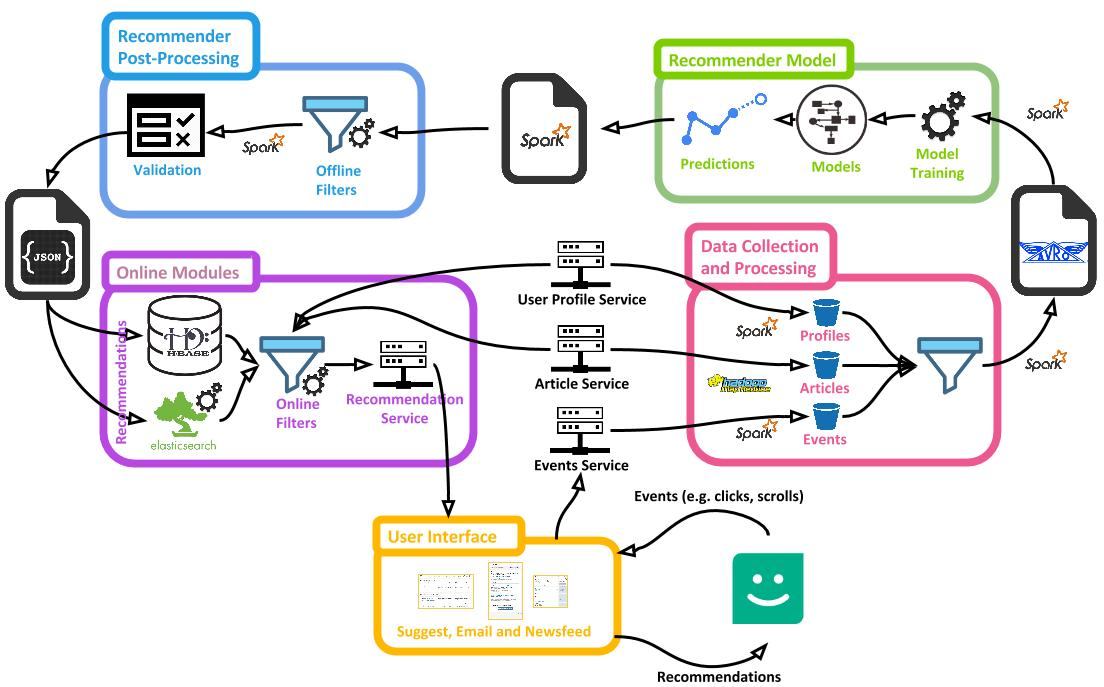
\includegraphics[scale=0.2]{images/mendeley.jpeg}
   \end{center}
\end{column}
\begin{column}{0.35\textwidth}
    \begin{tcolorbox}[colback=info!5,colframe=info!80,title=]
    \begin{small}
    Машинное обучение -- небольшая часть рекомендательного сервиса. Другие компоненты часто требуют не меньше усилий.
    \end{small}
    \end{tcolorbox}
\end{column}
\end{columns}

\footnote{Ссылки:
\href{https://hadoop.apache.org/}{Hadoop} +
\href{https://spark.apache.org/}{Spark} +
\href{https://hbase.apache.org/}{HBase} +
\href{https://www.elastic.co/what-is/elasticsearch}{Elasticsearch}
}

\end{frame}

\begin{frame}{Обработка данных под высокой нагрузкой / Netflix (2013) \cite{NFLX}}

\begin{columns}
\begin{column}{0.6\textwidth}
   \begin{center}
		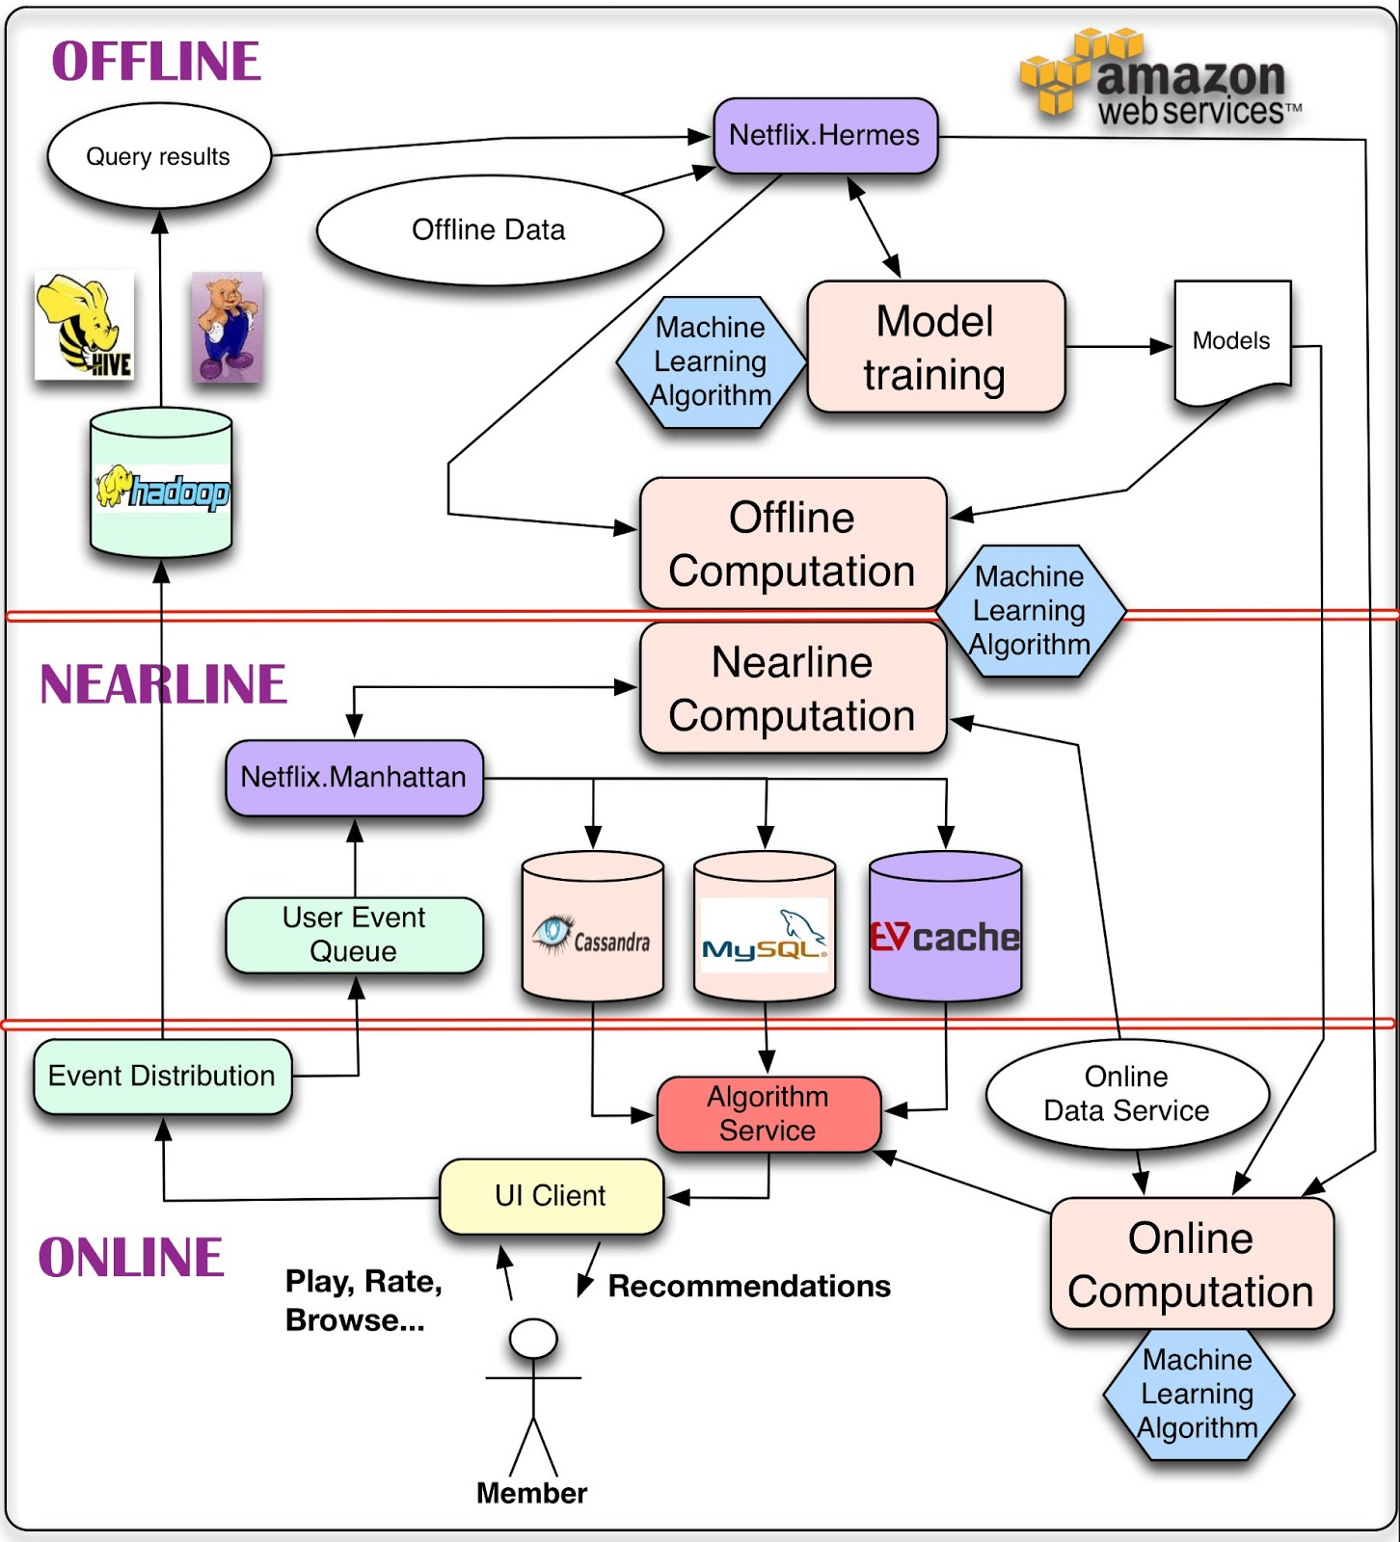
\includegraphics[scale=0.1]{images/netflix.png}
   \end{center}
\end{column}
\begin{column}{0.35\textwidth}
    \begin{small}
    \begin{tcolorbox}[colback=info!5,colframe=info!80,title=]
    Двигаясь от offline к real-time, мы можем быстрее реагировать на изменения контекста. При этом возникают ограничения на сложность алгоритмов.
    \end{tcolorbox}
    \end{small}
\end{column}
\end{columns}

\footnote{Ссылки:
\href{https://cassandra.apache.org/_/index.html}{Cassandra}
}


\end{frame}

\begin{frame}{Рекомендации айтемов из больших каталогов / Youtube (2016) \cite{YTBE}}
% Enormous action space, context
\begin{columns}
\begin{column}{0.6\textwidth}
   \begin{center}
		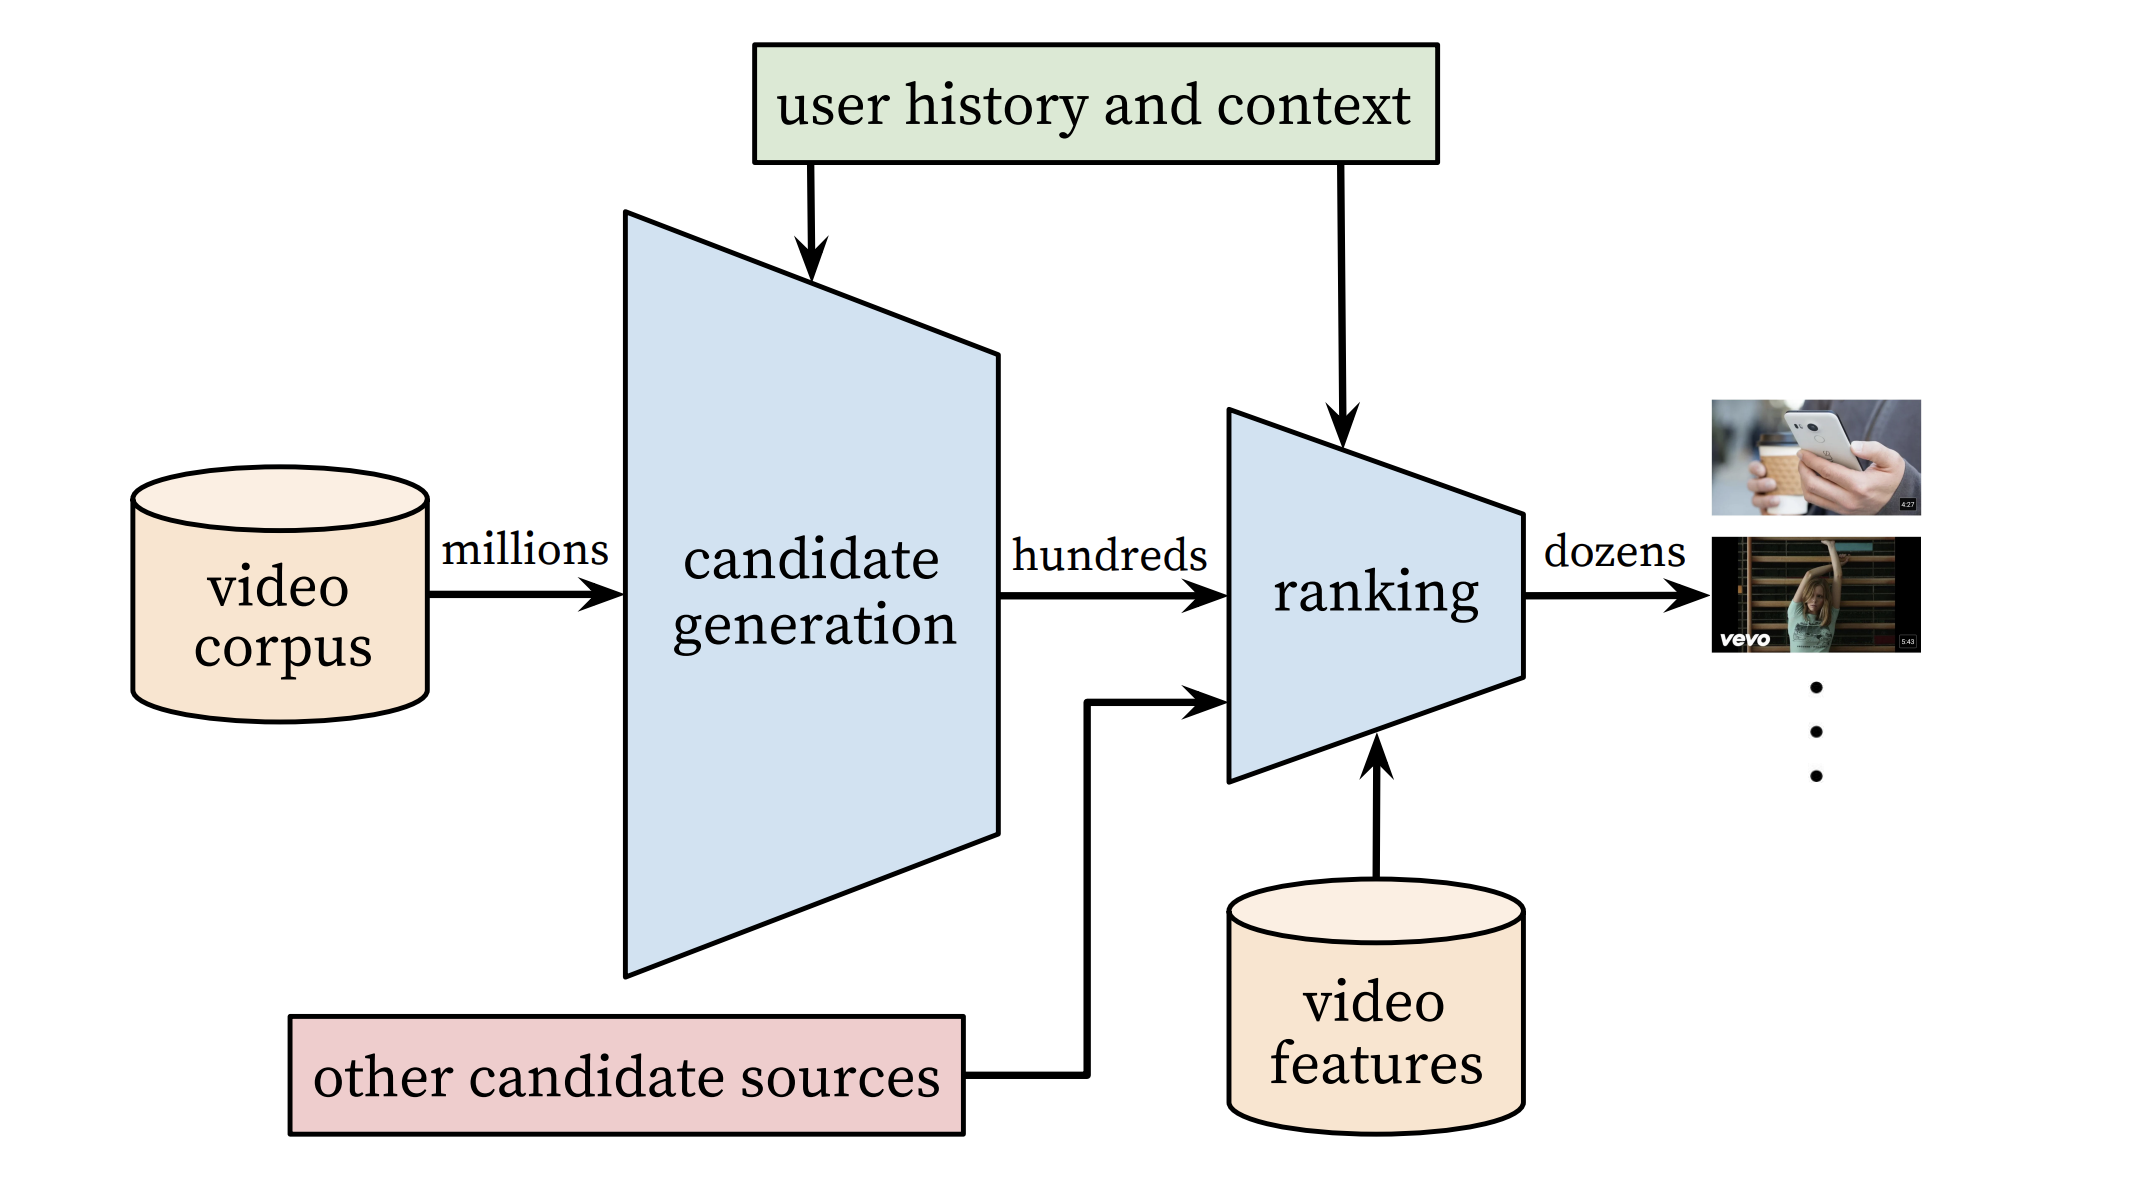
\includegraphics[scale=0.25]{images/youtube.png}
   \end{center}
\end{column}
\begin{column}{0.35\textwidth}
   \begin{small}
    \begin{tcolorbox}[colback=info!5,colframe=info!80,title=]
    Айтемов так много, что учесть {\bf полный контекст} не может даже Google. Для быстрого отбора кандидатов применяются грубые фильтры.
    \end{tcolorbox}
    \end{small}
\end{column}
\end{columns}

\end{frame}

\begin{frame}{Загадка}

Что общего между
\begin{itemize}
\item населением городов
\item количеством друзей у пользователей в социальной сети
\item размерами лесных массивов
\item количеством прослушиваний песен в Spotify
\end{itemize}

\end{frame}

\begin{frame}{Power law}

\[
p(x) = \frac{C} {x^{\alpha}}, \quad x > x_{min}
\]

\begin{center}

\includegraphics[scale=0.25]{images/longtail.png}

Правило 80/20
\end{center}

\end{frame}

\begin{frame}{Холодный старт и длинный хвост / Spotify (2016) \cite{SPTF}}
% Long tail, coldstart
\begin{columns}
\begin{column}{0.6\textwidth}
   \begin{center}
		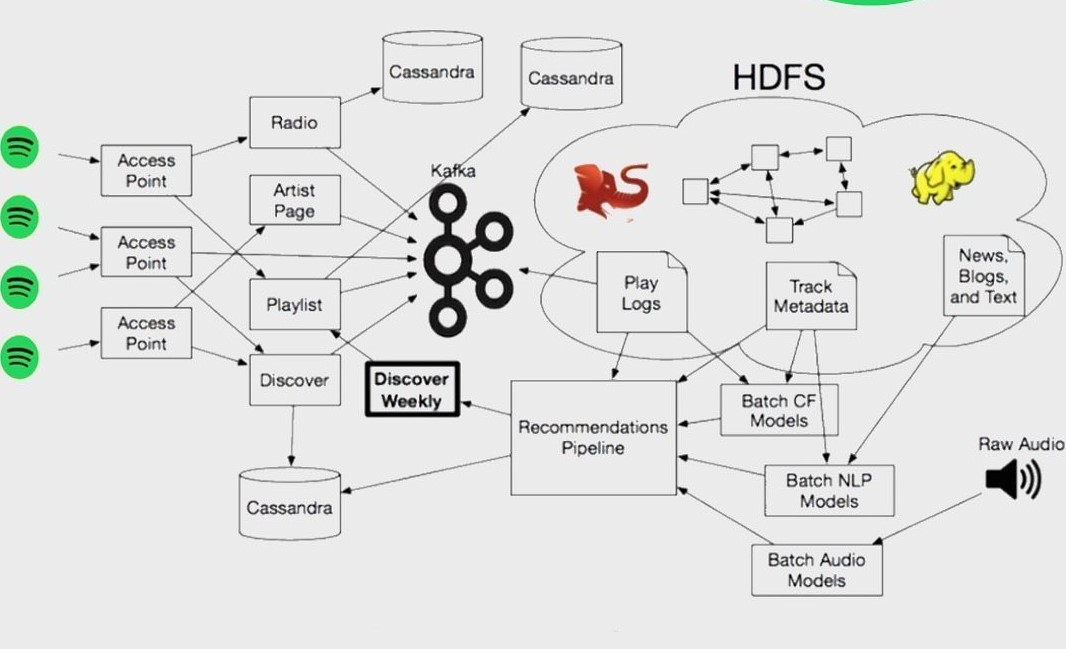
\includegraphics[scale=0.31]{images/spotify.jpeg}
   \end{center}
\end{column}
\begin{column}{0.35\textwidth}
\begin{small}
    \begin{tcolorbox}[colback=info!5,colframe=info!80,title=]
    Холодные айтемы и пользователи будут всегда. Использование контента - один из вариантов решения проблемы
    \end{tcolorbox}
\end{small}
\end{column}
\end{columns}

\footnote{Ссылки:
\href{https://kafka.apache.org/}{Кafka}
}

\end{frame}

\begin{frame}{Несоответствие таргетов моделей и business-value / TikTok (2020) \cite{TIK}}
% Intangible objectives, content, exploration/authors!
\begin{columns}
\begin{column}{0.6\textwidth}
   \begin{center}
		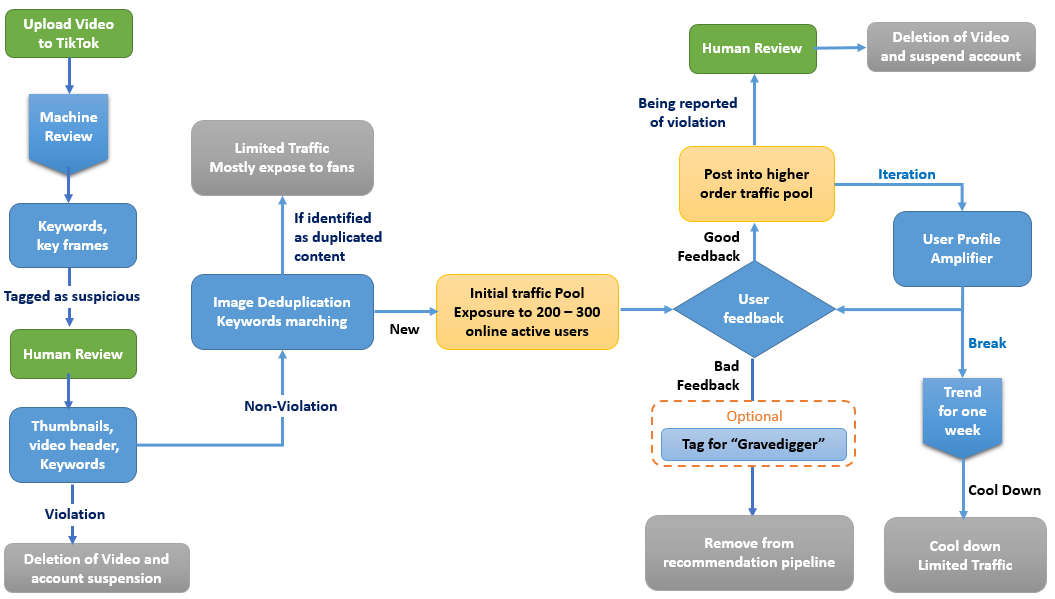
\includegraphics[scale=0.24]{images/tiktok.png}
   \end{center}
\end{column}
\begin{column}{0.35\textwidth}
    \begin{small}
    \begin{tcolorbox}[colback=info!5,colframe=info!80,title=]
    Потребности людей нельзя упаковать в удобную метрику. Кроме машинного обучения  в рекомендательных сервисах приходится исполтзовать пре- и пост-процессинг, чтобы гарантировать business-value.
    \end{tcolorbox}
    \end{small}
\end{column}
\end{columns}

\end{frame}

\begin{frame}{Как в действительности выглядит архитектура RS}

\begin{center}
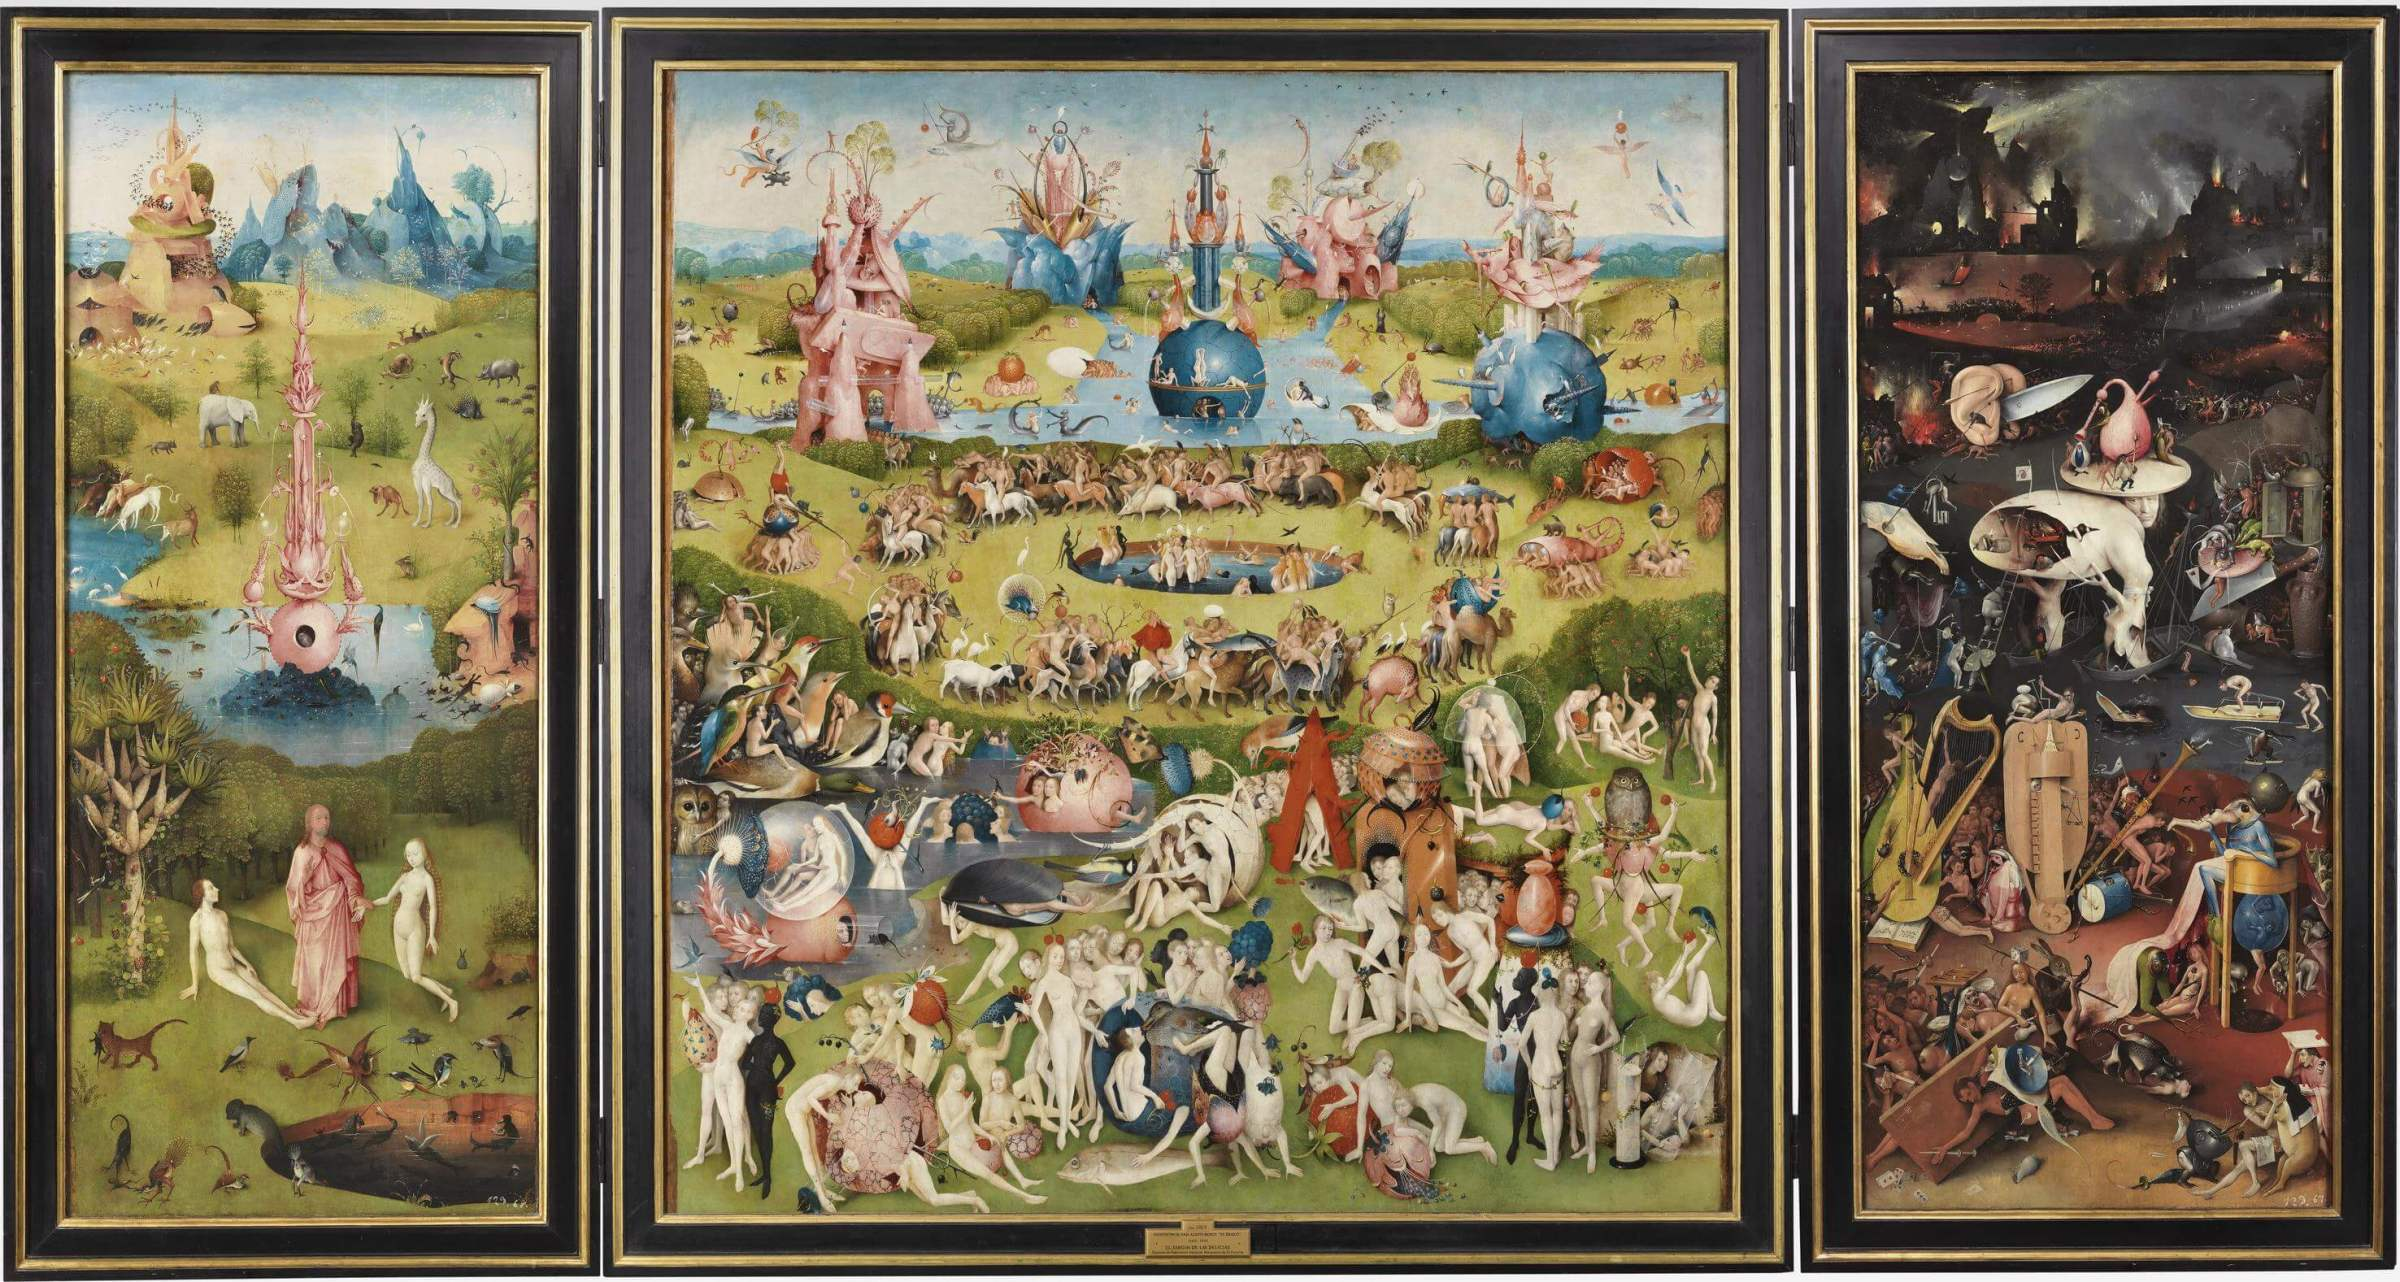
\includegraphics[scale=0.15]{images/bosch.jpeg}
\end{center}

\end{frame}

\begin{frame}{Какие сложности учитывает архитектура RS}

\begin{itemize}
\item Высокая нагрузка рекомендательных сервисов
\item Большие каталоги айтемов
\item Холодный старт пользователей и айтемов
\item Несоответествие business-value и метрик оптимизации
\end{itemize}

\end{frame}

\begin{frame}{Какие технические средства могут понадобиться}

\begin{itemize}
\item Отказоустойчивые продакшен-сервисы (HBase, Cassandra, Elasticsearch)
\item Передача данных (kafka)
\item Хранение данных (Hadoop HDFS)
\item Batch обработка данных (Spark)
\item Потоковая обработка данных (Kafka, Spark Streaming)
\end{itemize}

\end{frame}

\section{Метрики и эксперименты}

\begin{frame}{Netflix 2010-2021 \cite{NETFLIXAB}}

\begin{columns}
\begin{column}{0.45\textwidth}
   \begin{center}
		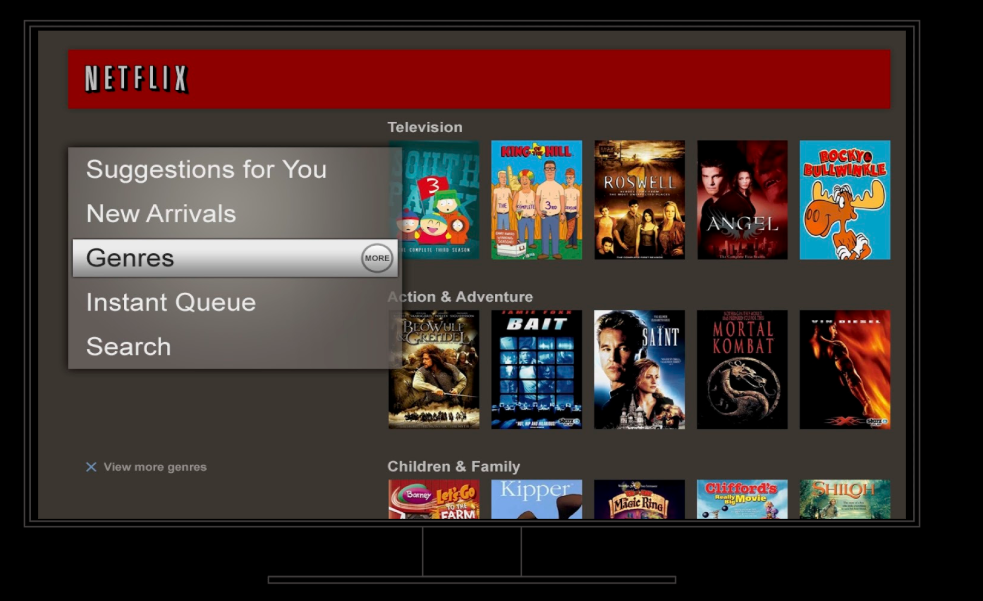
\includegraphics[scale=0.15]{images/netflix-2010.png}
   \end{center}
\end{column}
\begin{column}{0.45\textwidth}
   \begin{center}
		\includegraphics[scale=0.12]{images/netflix-2021.png}
   \end{center}
\end{column}
\end{columns}

\end{frame}

\begin{frame}{}

Хотим принимать решения на основе данных $\rightarrow$ 

\qquad Начинаем собирать метрики $\rightarrow$ 

\qquad \qquad Разрабатываем инструменты для принятия решений

\begin{center}
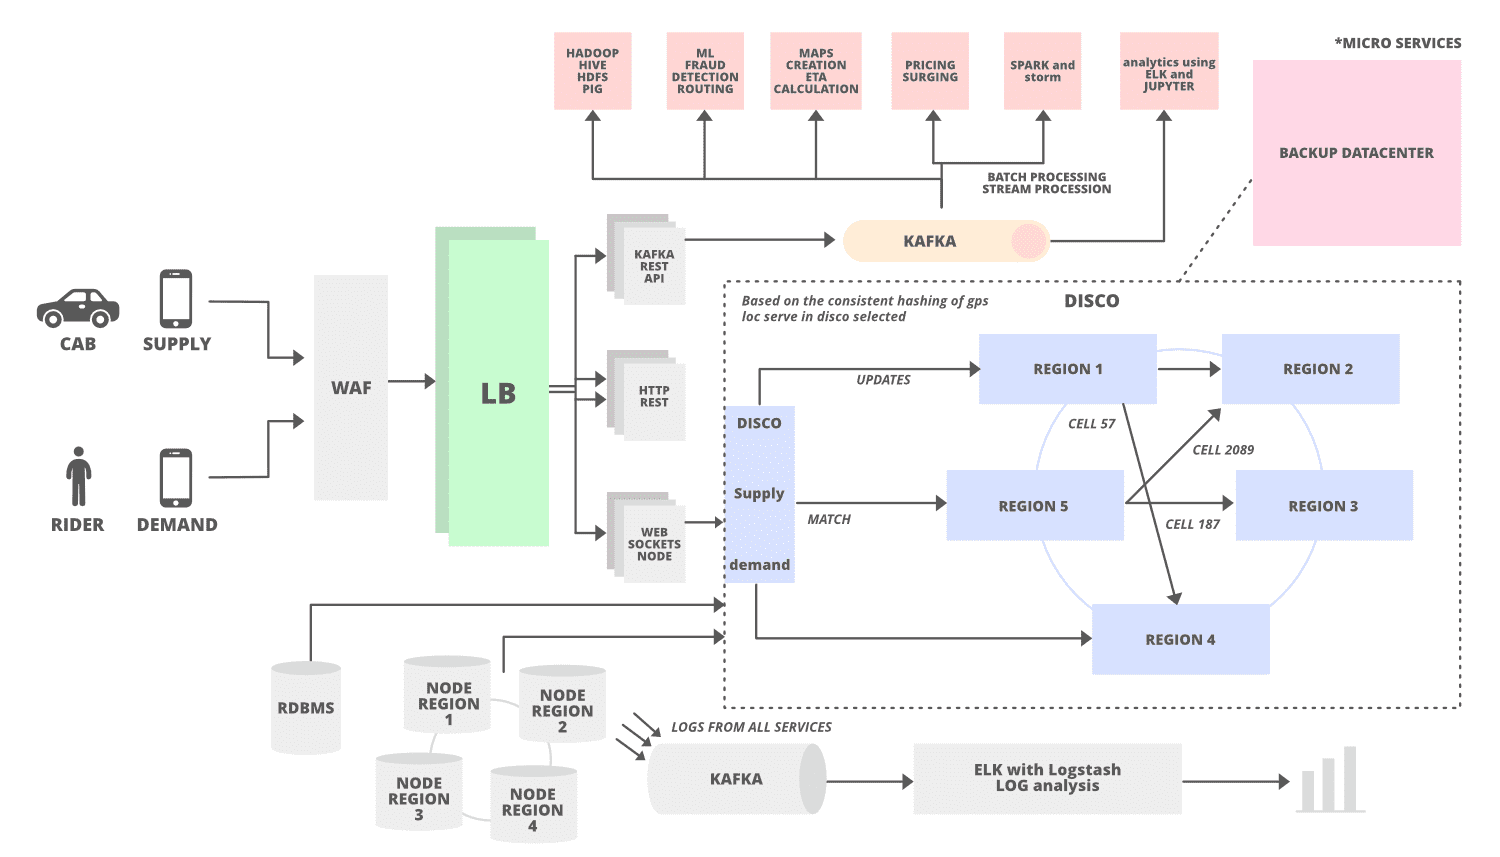
\includegraphics[scale=0.18]{images/uber.png}
\end{center}

\footnote{Ссылки: ELK = Elasticsearch + \href{https://www.elastic.co/kibana/}{Kibana}}

\end{frame}

\begin{frame}{Наивный подход к измерению эффекта}
\begin{center}
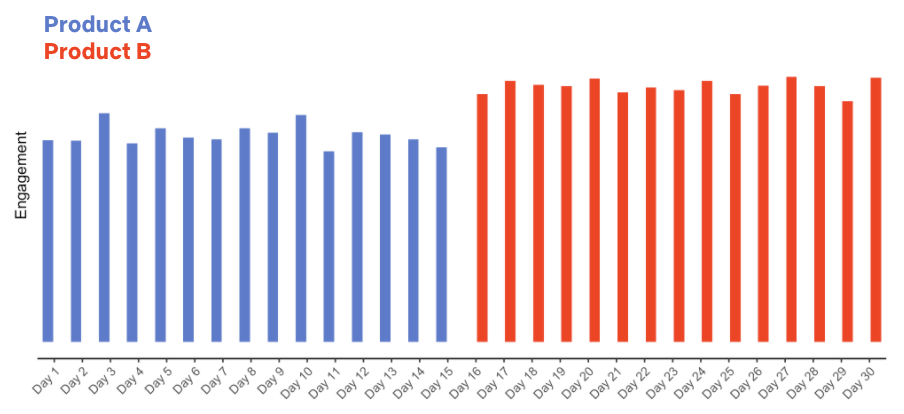
\includegraphics[scale=0.3]{images/noexp.png}
\end{center}
\end{frame}

\begin{frame}{}

\begin{tcolorbox}[colback=info!5,colframe=info!80,title=Задача]
Какой {\bf причинно-следственный эффект} на распределение целевой метрики окажет выбранное воздействие $T$?
\end{tcolorbox}

\vfill

\begin{tcolorbox}[colback=warn!5,colframe=warn!80,title=Фундаментальная Проблема Causal Inference]
Для конкретного пользователя невозможно вычислить causal effect напрямую, потому что нельзя пронаблюдать значение целевой переменной при более чем одном значении $T$\footnote{Без дополнительных предположений эту проблему не решить \cite{GELMAN}}
\end{tcolorbox}

\end{frame}

\begin{frame}{Фреймворк Potential Outcomes}

Воздействие на $i$ пользователя:
\[
T_i = \begin{cases}
0, \quad \text{если показываем сontrol} \\
1, \quad \text{если показываем treatment}
\end{cases}
\]

Соответствующие потенциальные исходы:
\[
y_i^0 \text{ и } y_i^1
\]

Требуется оценить:
\begin{tcolorbox}[colback=info!5,colframe=info!80,title=Average Treatment Effect,center,width=6cm,center title]
\[
ATE = E \left[ y_i^1 - y_i^0 \right]
\]
\end{tcolorbox}

\end{frame}

\begin{frame}{Randomized Controlled Experiment}

\begin{tcolorbox}[colback=info!5,colframe=info!80,title=Схема эксперимента]
Все доступные пользователи независимо друг от друга случайным образом распределяются в control либо treatment с одинаковой вероятностью
\end{tcolorbox}

\end{frame}

\begin{frame}{\phantom{Предположения RCE}}

\begin{tcolorbox}[colback=warn!5,colframe=warn!80,title=Предположение 1: ]
Можно оценить значение некоторой характеристики для всей популяции, имея выборку из этой популяции.
\end{tcolorbox}

\vfill

\begin{tcolorbox}[colback=warn!5,colframe=warn!80,title=Предположение 2: Stable Unit Treatment Value Assumption]
Потенциальные исходы для каждого пользователя зависят только от свойств этого пользователя, но не свойств и исходов других пользователей.
\end{tcolorbox}

\end{frame}

\begin{frame}{Оцениваем ATE в RCE}

\[
ATE = E[y_i^1 - y_i^0] = E[y_i^1] - E[y_i^0] \sim \text{avg}_{i \in T}(y_i^1) - \text{avg}_{i \in C}(y_i^0) = \bar y_1 - \bar y_0
\]

\begin{itemize}
\item нужно оценить две характеристики -- $E[y_i^0]$ и $E[y_i^1]$, поэтому используем выборки $C$ и $T$
\item проще всего сделать оценку, если выборка несмещенная
\item чем больше данных, тем точнее оценка
\end{itemize}

\end{frame}

\begin{frame}{}

\begin{center}
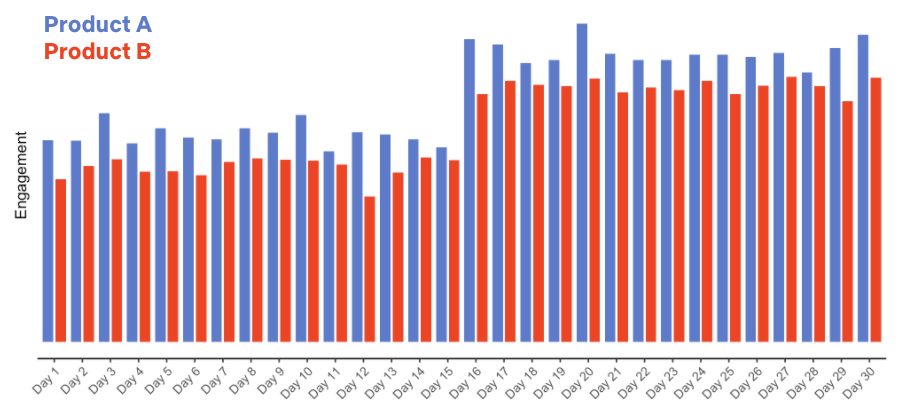
\includegraphics[scale=0.3]{images/yesexp.png}
\end{center}

\end{frame}

\begin{frame}{Доверительный интервал на ATE}

Доверительный интервал $(L, U)$ с уровнем доверия $\alpha$:
\[
P(L < \theta < U) = 1 - \alpha
\]

Формула Уэлча:
\[
\bar y_1 - \bar y_0 \pm t_{\alpha/2,r} \sqrt{\frac{s_1^2}{n_1} + \frac{s_0^2}{n_0}}, \quad
r = \frac{ \left( \frac{s_1^2}{n_1} + \frac{s_0^2}{n_0} \right)^2 }{ \frac{s_1^4}{n_1^2 (n_1 - 1)} + \frac{s_0^4}{n_0^2 (n_0 - 1)} }
\]
Где:
\begin{itemize}
\item $n_1$ и $n_0$ -- количество пользователей в treatment и control
\item $s_1^2$ и $s_0^2$ -- оценки дисперсии метрики в treatment и control
\item $t_{\alpha/2,r}$ -- табличное значение для $r$ степеней свободы
\end{itemize}

\end{frame}

\begin{frame}{На практике}

\begin{itemize}

\item Перед запуском
\begin{itemize}
\item Выбираем ключевую метрику, несколько сопутствующих метрик и контролируем, что не ``уронили'' важные
\item Выбираем длительность эксперимента, оценивая мощность теста :D
\end{itemize} 

\item При анализе
\begin{itemize}
\item Метрики распределены по-разному: нужно подбирать подходящие тесты
\item Используются методы снижения дисперсии оценок (cuped, diff-in-diff)
\end{itemize}

\end{itemize}

\vfill

\begin{tcolorbox}[colback=info!5,colframe=info!80]
Если вы попали в компанию, в которой есть культура принятия решений на основе данных -- сохраняйте ее всеми силами. Если нет -- пропагандируйте.
\end{tcolorbox}

\end{frame}

\begin{frame}{Сложности RCE в индустриальных рекомендерах \cite{FACEBOOK}}

\begin{itemize}[<+->]
\item Как выбрать Самую Главную Метрику (OEC)? 
\item Как оценить долгосрочный эффект?
\item Разный эффект на разных сегментах пользователей
\item Отсутствие культуры экспериментирования
\item Масштабирование платформы для экспериментов
\item Сетевые эффекты
\item Наложение эффектов от экспериментов
\end{itemize}

\end{frame}

\section{Итоги}

\begin{frame}

\begin{tcolorbox}[colback=info!5,colframe=info!80]
В основе рекомендательных сервисов лежит машинное обучение. При проектировании  нужно учитывать множество дополнительных факторов, например требования к скорости обработки данных, эффект длинного хвоста и возможность холодного старта.
\end{tcolorbox}
\vfill
\begin{tcolorbox}[colback=info!5,colframe=info!80]
A/B эксперимент -- надежный способ оценки эффекта от изменений в сервисе.
\end{tcolorbox}

\end{frame}

\begin{frame}[allowframebreaks]{Литература}
\bibliographystyle{amsalpha}
\bibliography{references.bib}
\end{frame}

\end{document}
